% ! TeX root = main.tex
\documentclass[9pt, aspectratio=169]{beamer}
\usepackage[utf8]{inputenc}
\usepackage{multicol}
\usepackage{pgfpages}
\usepackage{roboto}
\usepackage{fontawesome5}
\usepackage[T1]{fontenc}
\usepackage{pdfcomment}
\title{Research directions for Aggregate Computing with
Machine Learning}
\author[G.Aguzzi]{
  \textbf{Gianluca Aguzzi}\inst{1}
}
\institute{
  \inst{1}
  \texttt{Alma Mater Studiorum} -- Università di Bologna, Cesena, Italy
}
\usetheme{material}
%& Theme
\usetheme{material}
\setbeamercolor{button}{bg=white,fg=accent}

\useLightTheme
\usePrimaryBlueGrey
\useAccentIndigo
%% Simplify document writing
%%\includeonly{slides/aggregate-and-sl.tex}
%% Document starts 
\begin{document}
\setbeamercovered{transparent=10}
\setbeamertemplate{itemize item}{\faDotCircle}

% ! TeX root = ...

\begin{frame}
  \begin{backgroundblock} 
    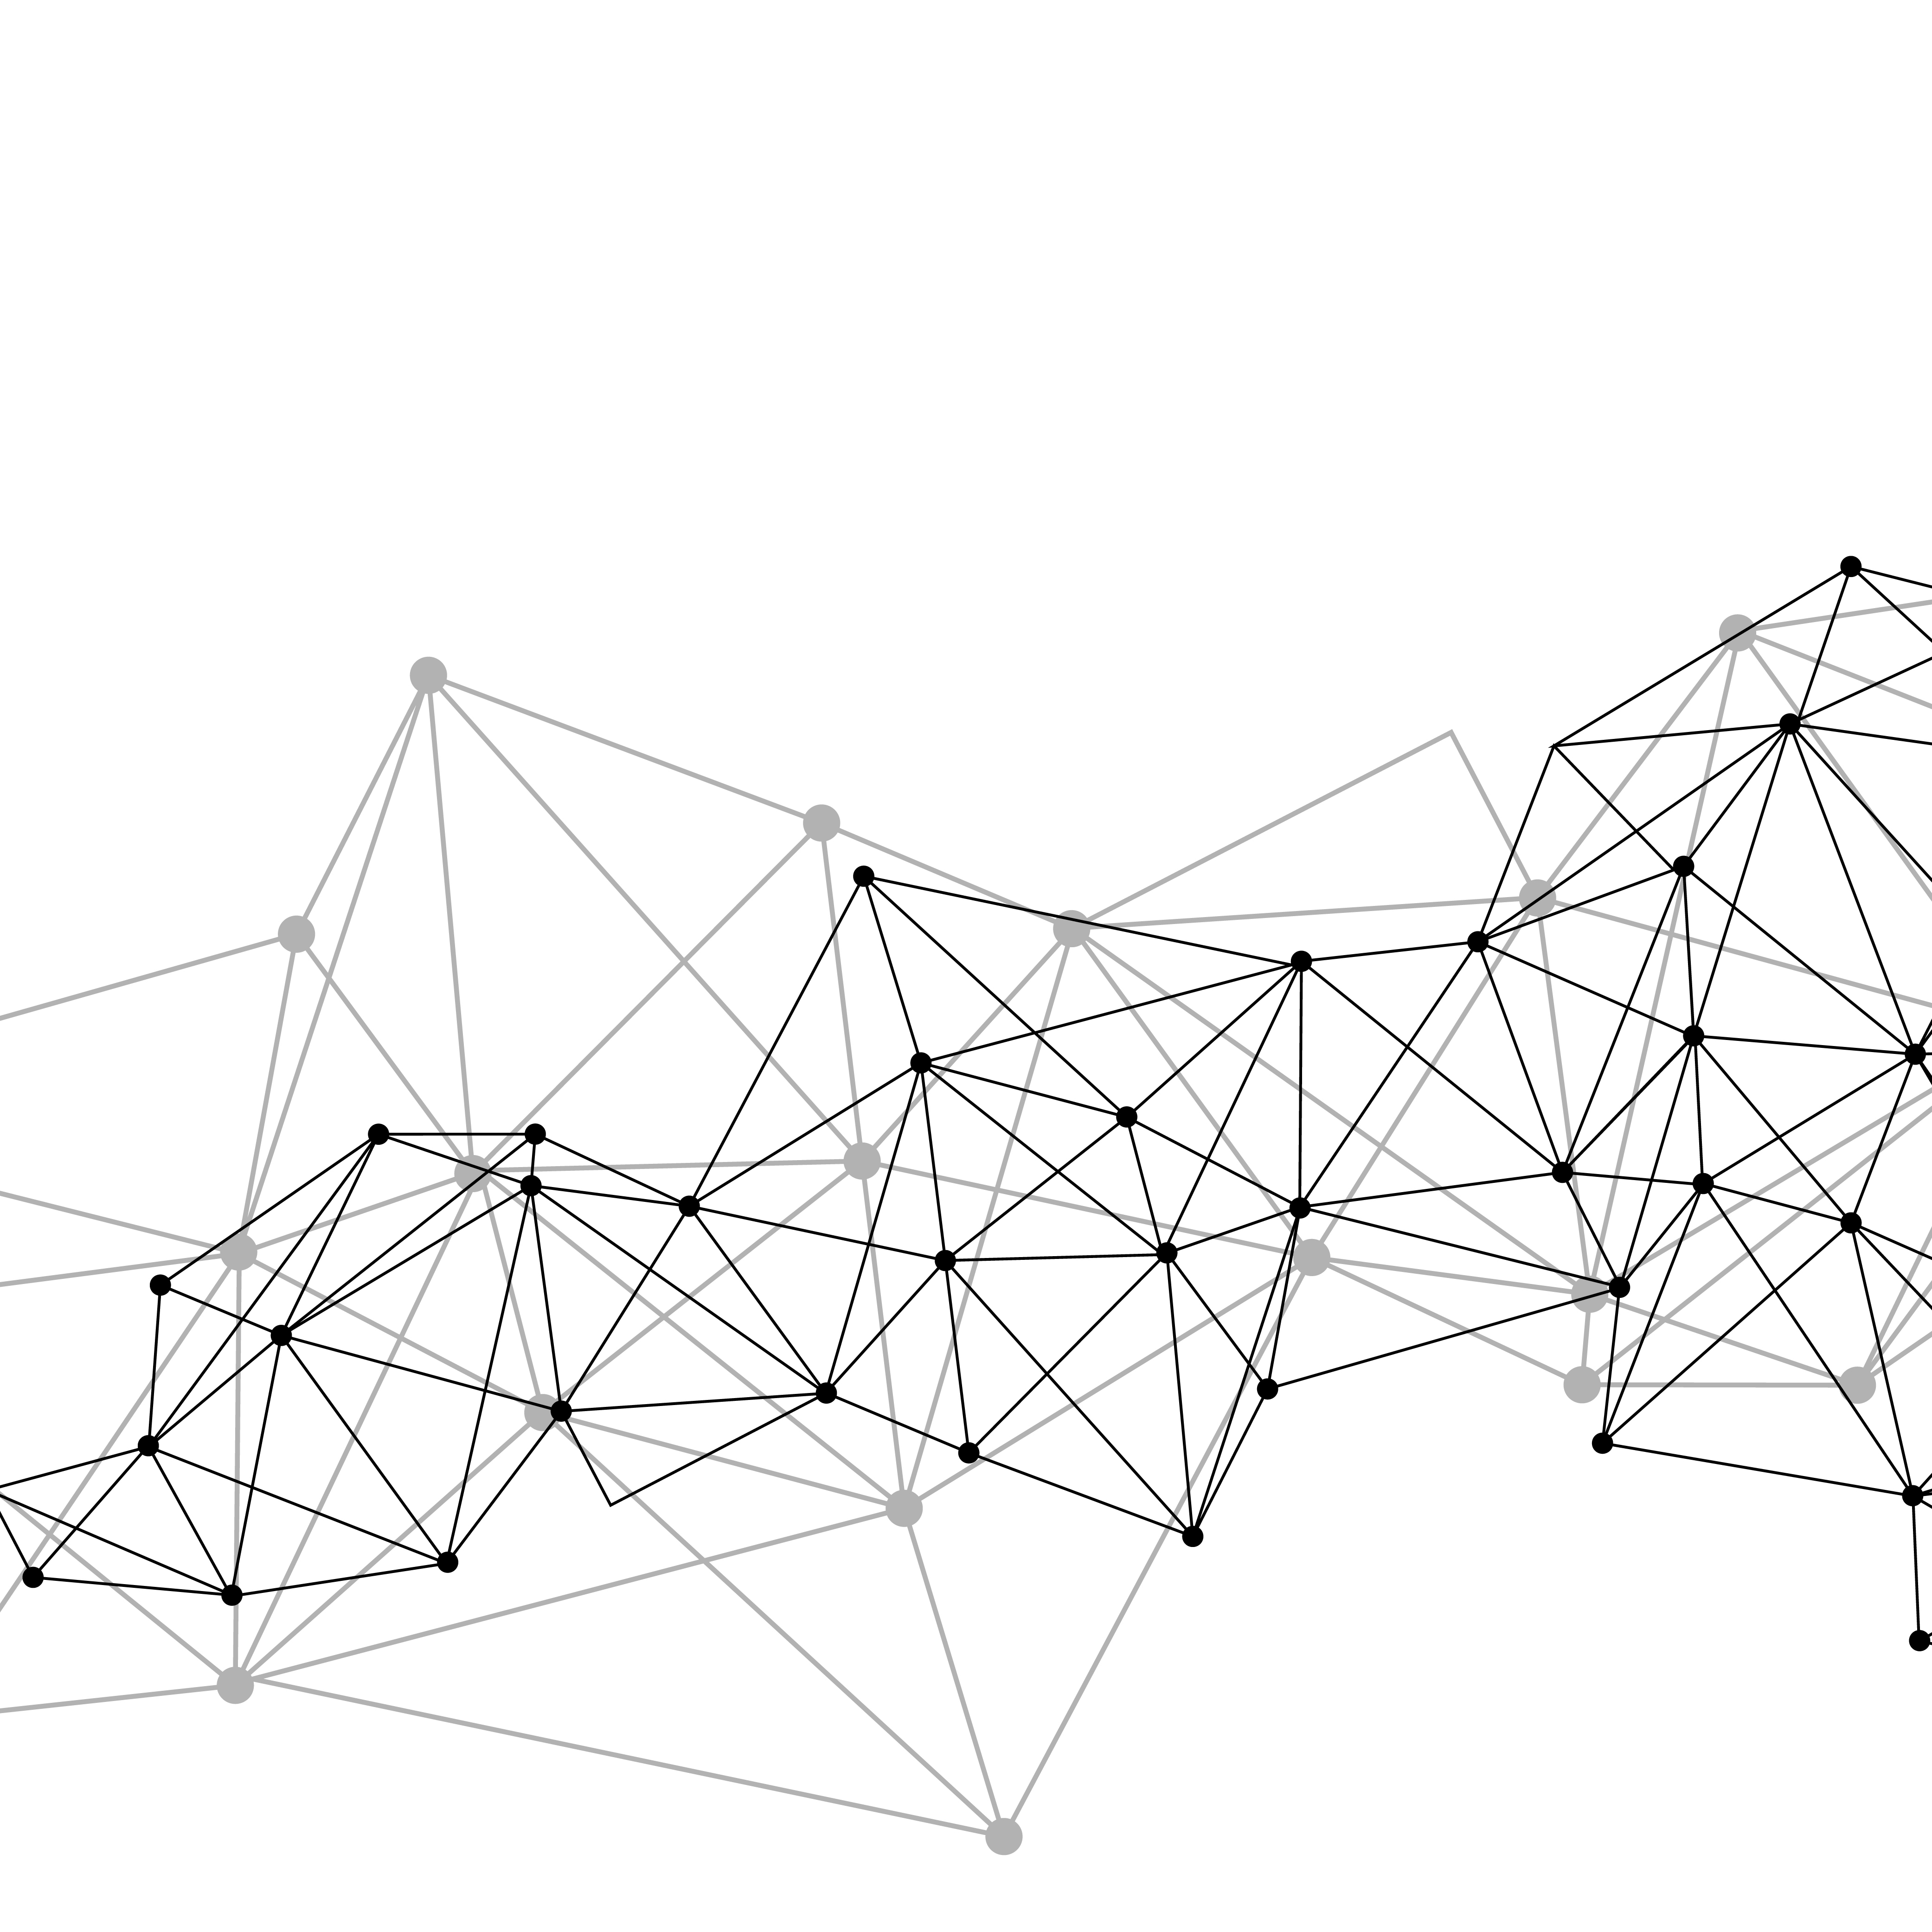
\includegraphics[width=\paperwidth]{img/main-background.jpg} 
  \end{backgroundblock} 
  \titlepage
  \pdfcomment{
    A brief introduction about who I am and my research goals
  }
\end{frame}

\section{Collective (Self-)Adaptive System}
% ! TeX root = ...

\begin{frame}{Background}
  \begin{backgroundblock} 
    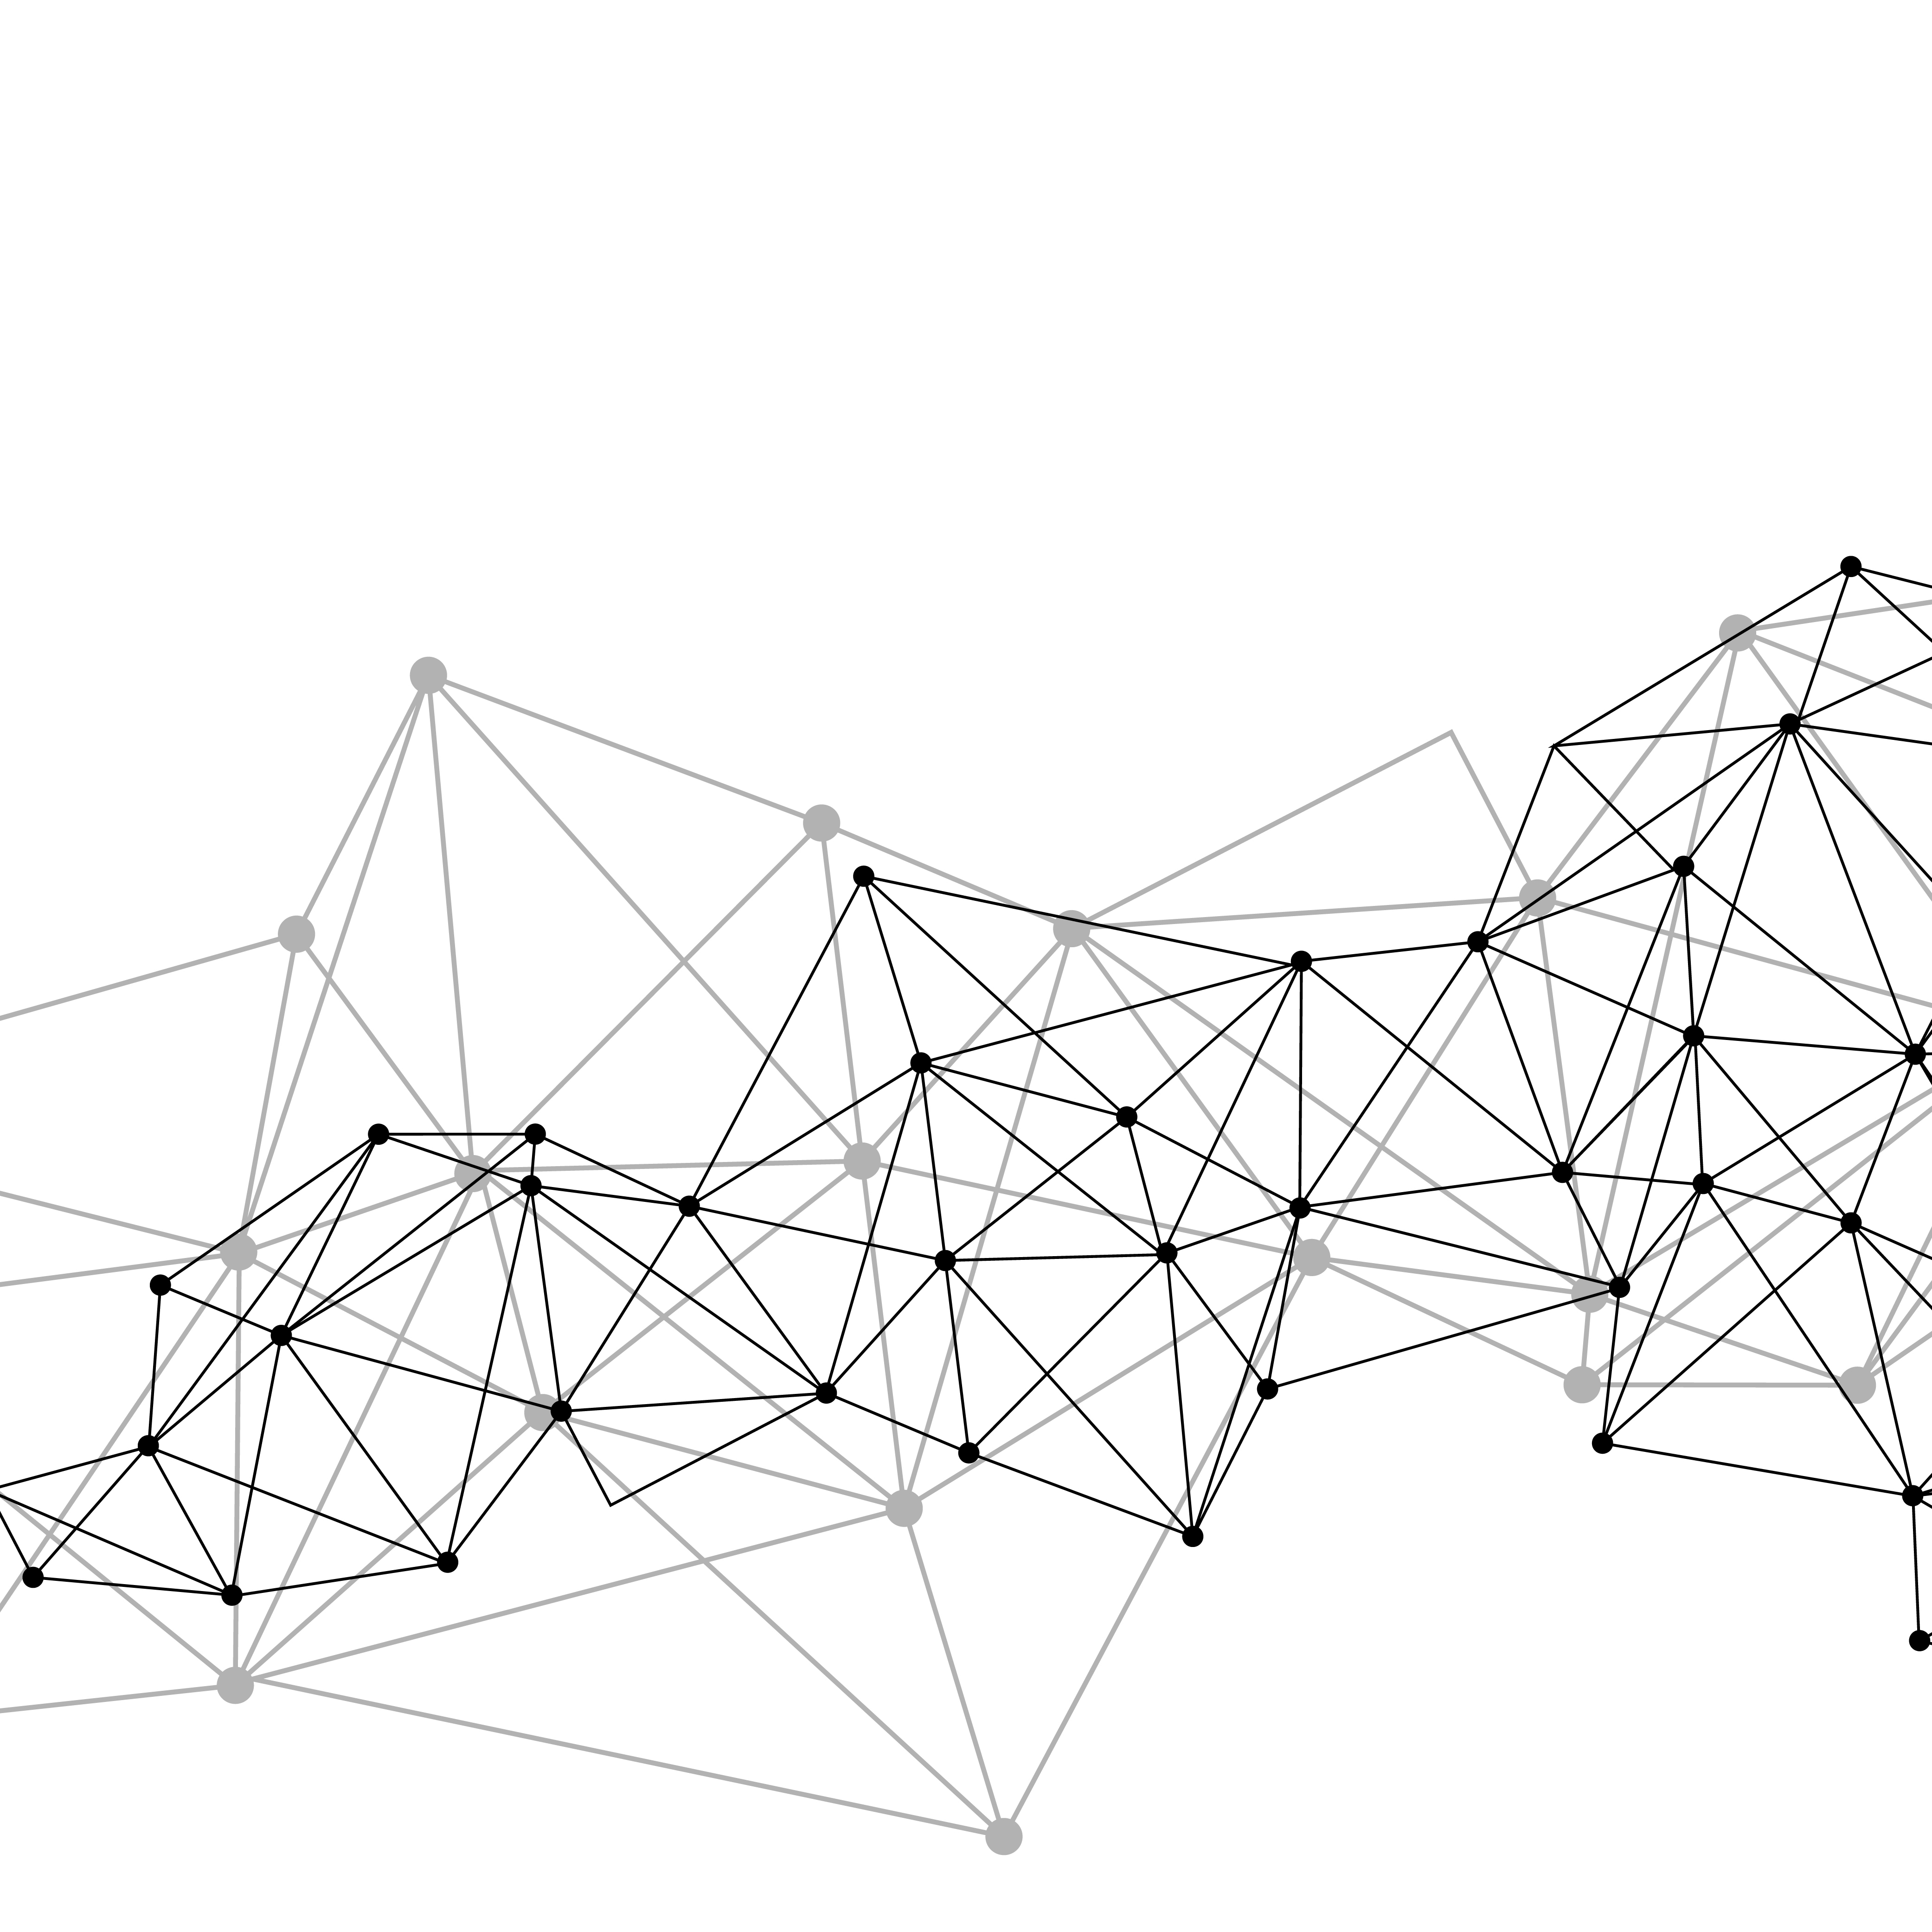
\includegraphics[width=\paperwidth]{img/main-background.jpg} 
  \end{backgroundblock} 
  \begin{card}[Collective (Self-)Adaptive Systems (\textbf{CSAS})]
    {
      \color{accent}
      Distributed and interconnected systems composed of multiple agents that can perform complex 
      tasks exhibiting robust collective behaviours while achieve system-wide and agent-specific goal. 
    }

  \pdfcomment{
    Our research effort consists of an engineering Collective (Self-)Adaptive System. 
    They can be defined as distributed and interconnected systems composed of multiple agents that can perform complex 
    tasks such as environmental data collection, search and rescue operations, and discovery of natural resources.
    So the collective exhibit robust behaviour while achieving system-wide and agent-specific goals.
    For years, there have been various approaches in the literature to deal with these systems. 
    In my research group, we focus on Aggregate Computing.
  }
  \end{card}
\end{frame}

\section{State of the art solution}
% ! TeX root = ...

\begin{frame}{Aggregate Computing}
  \begin{backgroundblock} 
    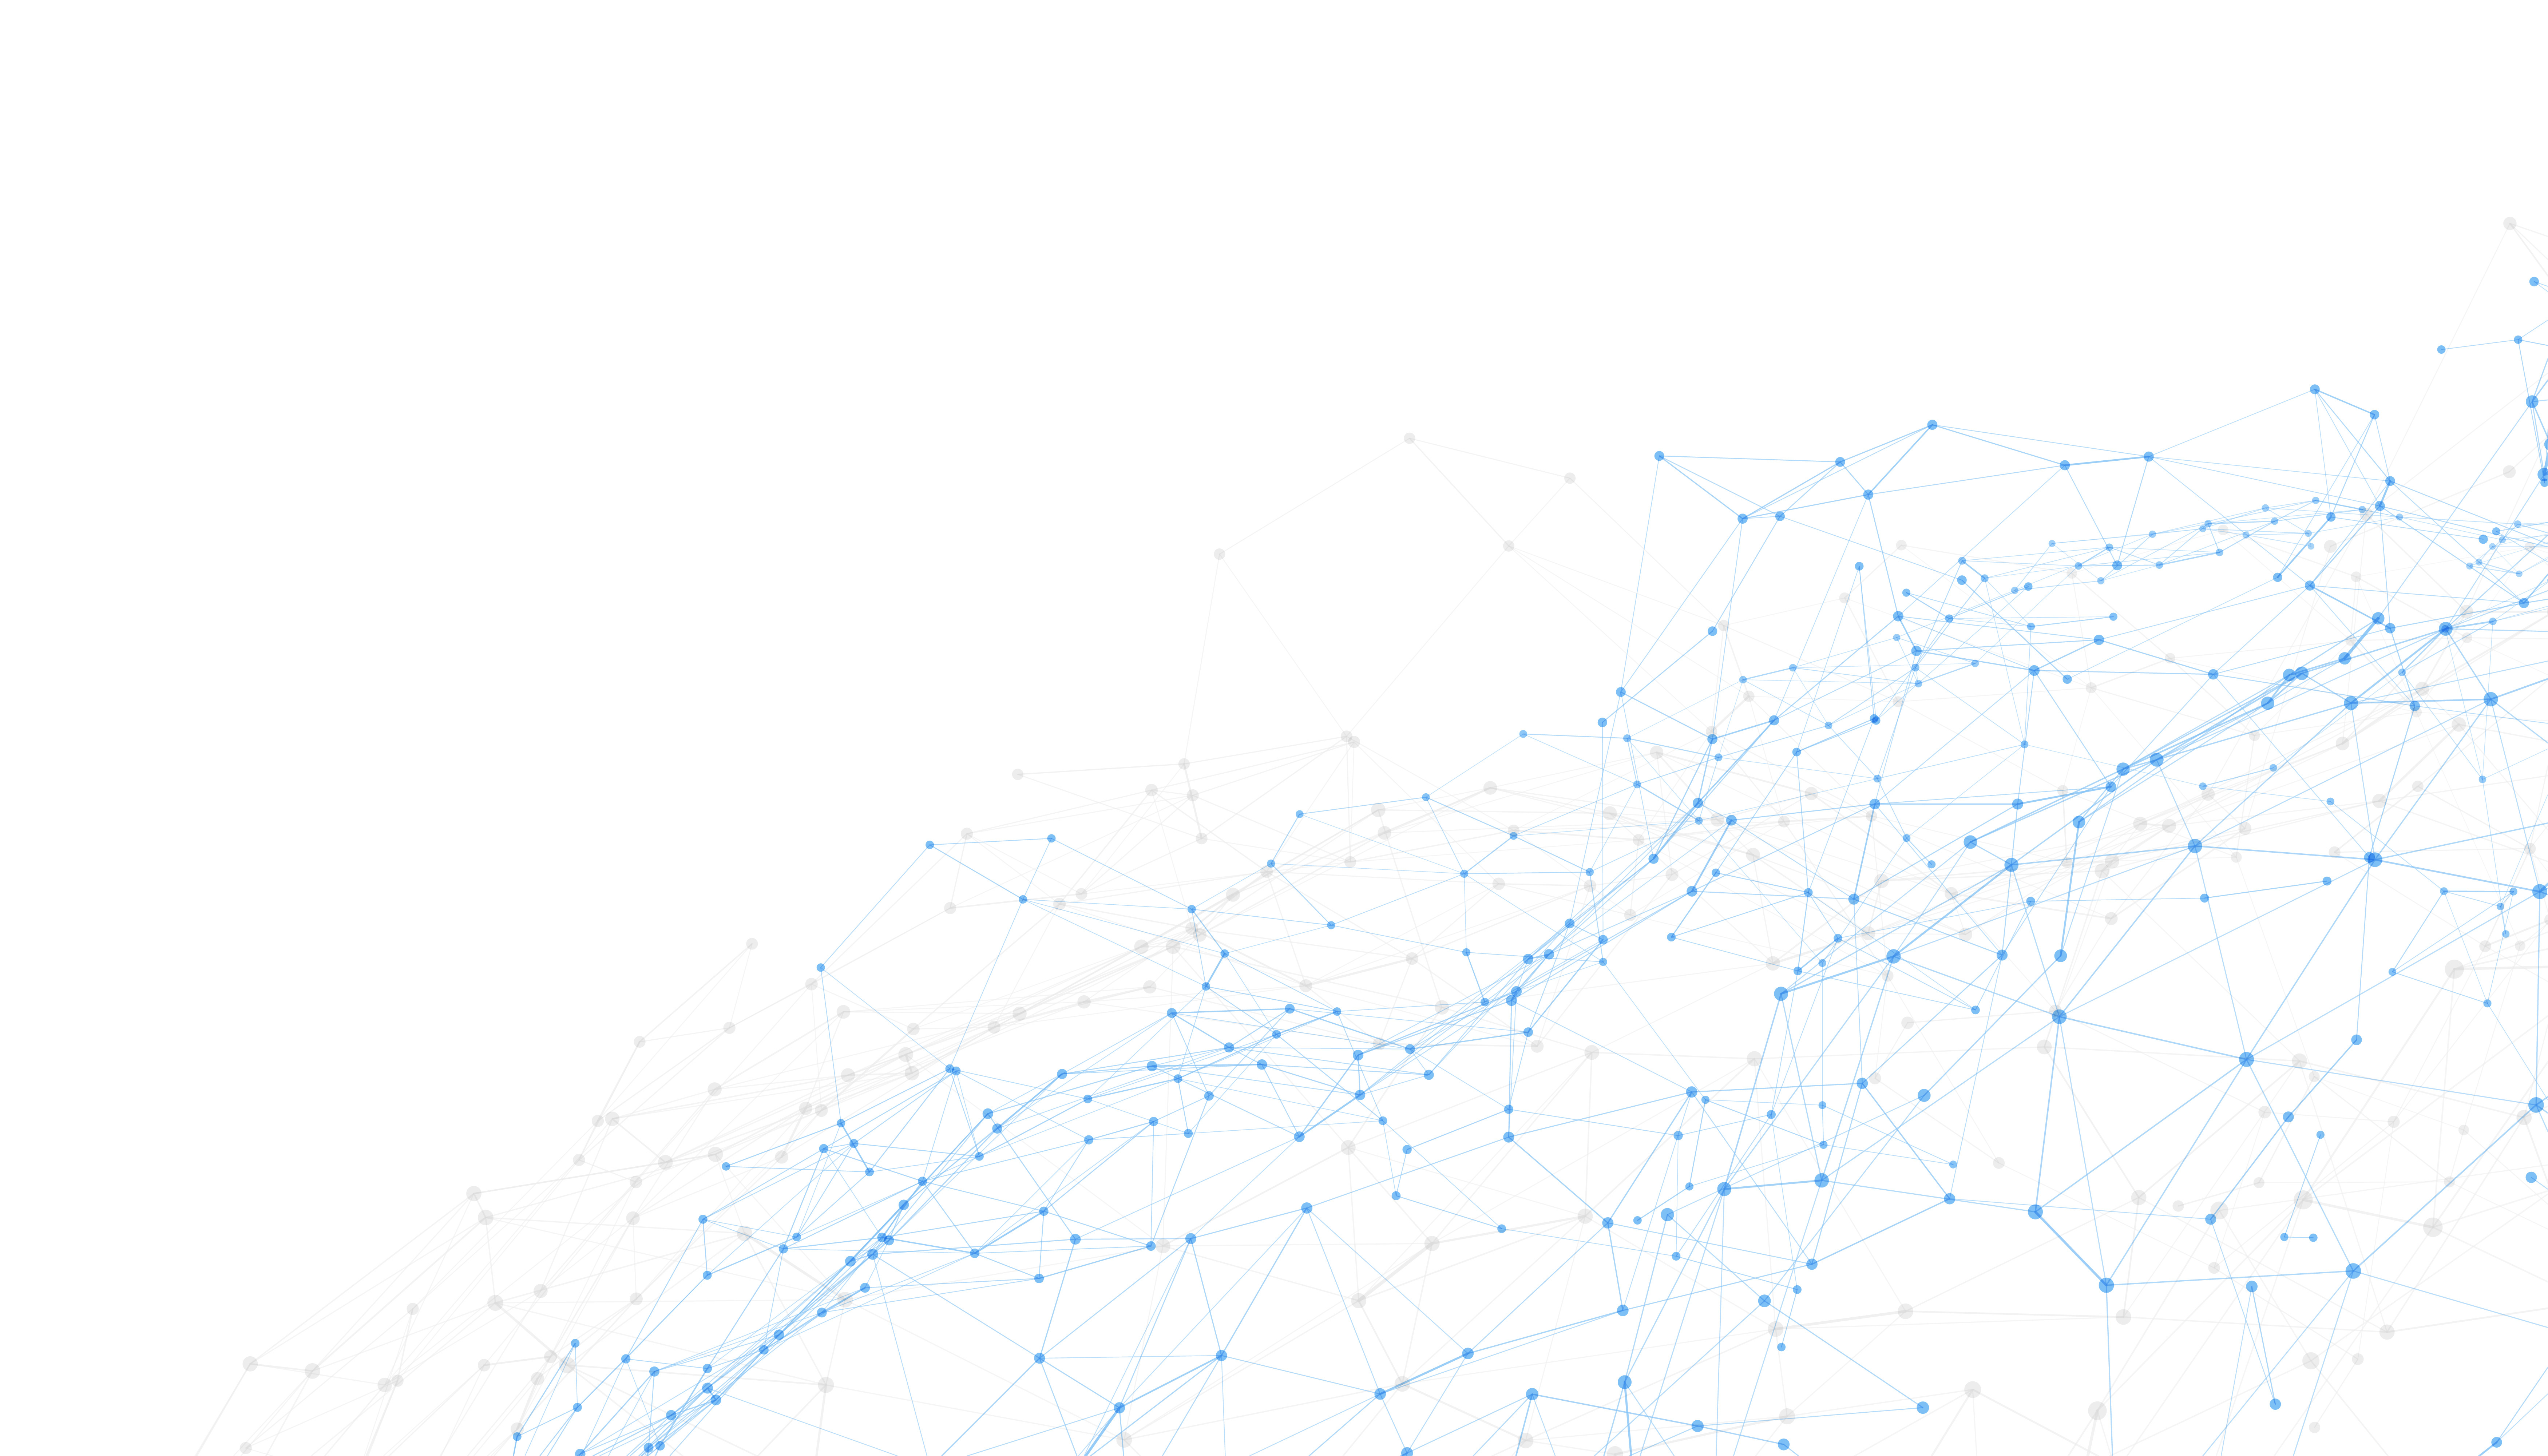
\includegraphics[width=\paperwidth]{img/aggregate-computing.jpg} 
  \end{backgroundblock} 
  \begin{card}
    \begin{itemize}
      \item <1-> A top-down global-to-local approach to express collective behaviour
      \item <2-> Rooted on \textit{field-calculus}
      \item <3-> Collective behaviour does not depends on system scale
      \item <4-> Used in various scenarios ranging from smart cities to crowd engineering
    \end{itemize}
  \end{card}
  \pause[5]
  \begin{cardRed}[\textbf{Problem} \faThumbsDown]
    \centering
    \textit{Building block design is hard}
  \end{cardRed}

  \pdfcomment{
    It is a top-down approach that makes it possible to coordinate large-scale, possibly heterogeneous, highly dynamic systems. 
    It mainly consists of manipulating a distributed data structure called Computational Field. 
    In contrast to swarm intelligent approaches, the idea here is to "program" the self-organisation by representing it as something like a first-class citizen of the language. 
    The program then can be split in each node, so that the collective behaviour can be easily scaled in very large systems (hundreds or thousands of nodes).
    A key advantage of this approach is its compositionality, which is inspired by functional programming.
    The paradigm is based on a small algebra called the field calculus, which expresses the minimal constructs that can be used to express any spatiotemporal computation.
    On top of this, we built intermediate-level abstractions, called Building-Block, which consist of the common patterns used in Aggregate Computing.
    We then used them to build domain-oriented applications to help developers express complex collective behaviour.
    Over the last ten/fifteen years, this methodology has grown rapidly. It is being used in many contexts such as crowd engineering, swarm robotics, and smart cities.
    Pragmatically, we see that it is not easy to develop building blocks that work well in different scenarios (e.g., high node mobility, uncertain environments).
    Sometimes it is a very tricky process of fine-tuning where we need to apply some constants to make our application work.
  }
\end{frame}
\begin{frame}{Machine Learning}
  \begin{backgroundblock} 
    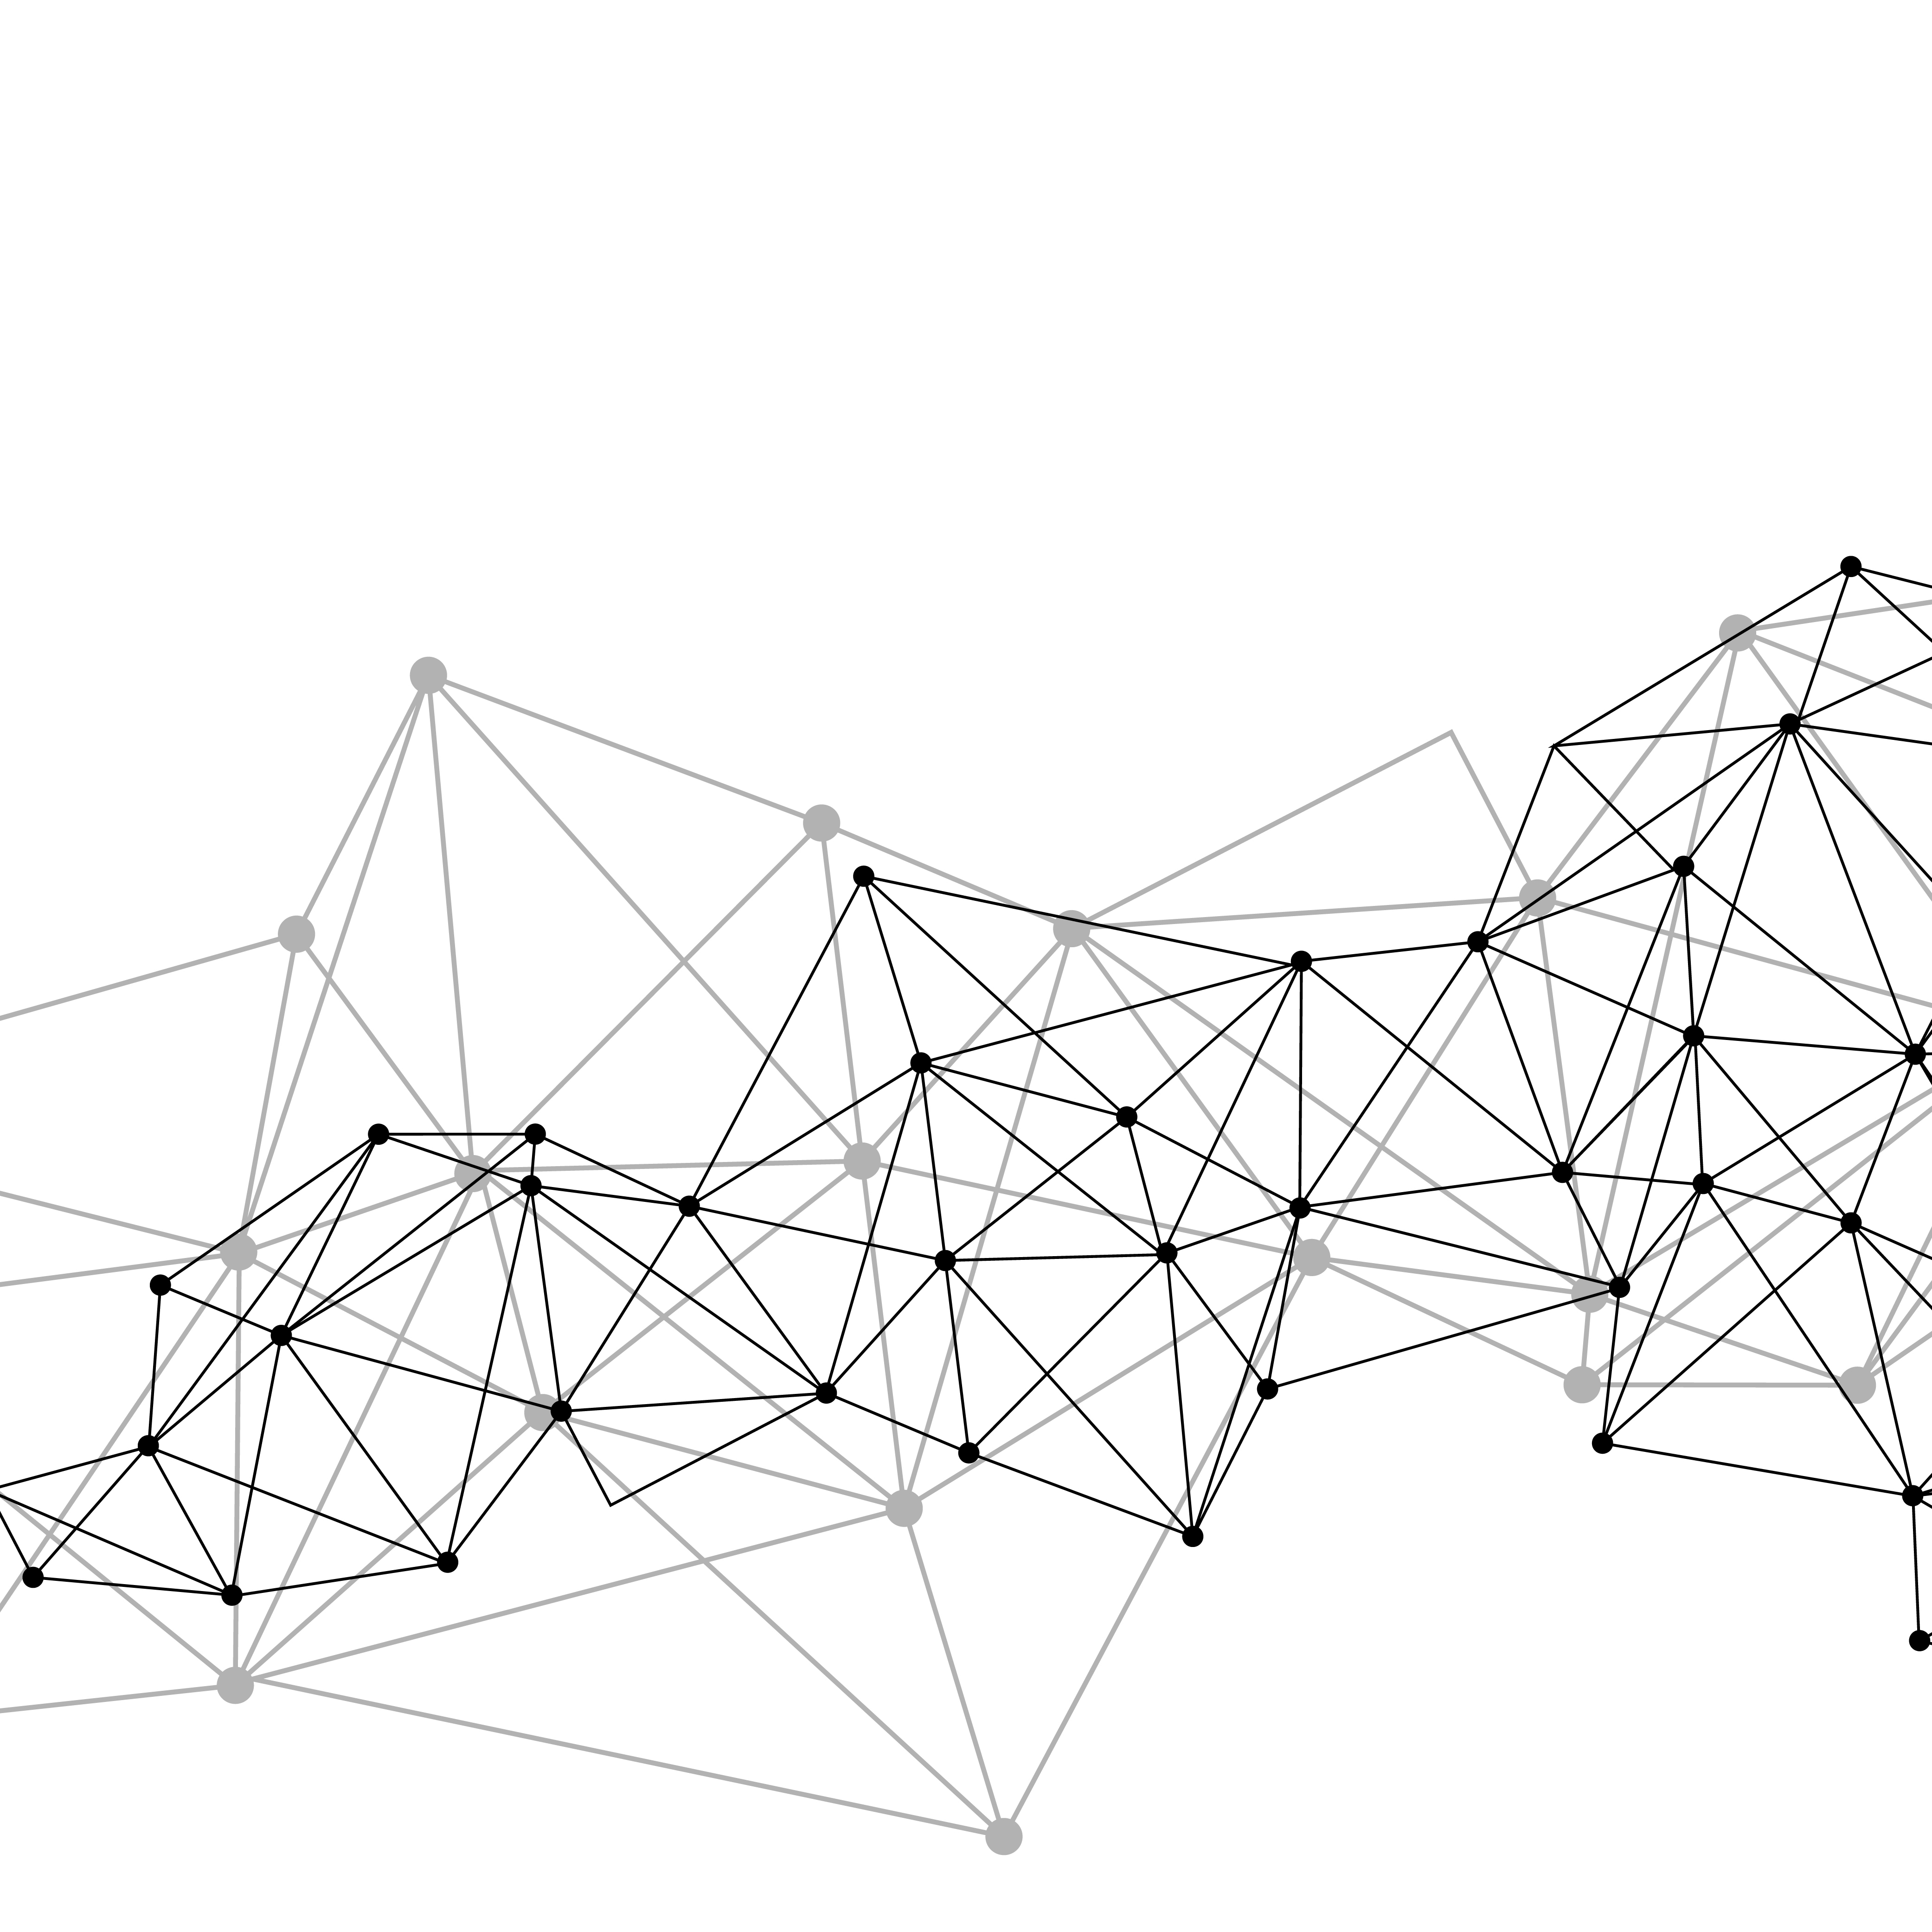
\includegraphics[width=\paperwidth]{img/main-background.jpg} 
  \end{backgroundblock} 
  \begin{card}{
    \begin{itemize}
      \item <1-> Enhance agents with \textit{some} learning capabilities 
      \item <2-> Learning improve adaptability, helping agent to act in uncertain environments
      \item <3-> Supervised Learning, Reinforcement Learning and Evolutionary Computing are typacally used in CSAS
    \end{itemize}
  }
  \end{card}
  \pause[4]
  \begin{cardRed}[\textbf{Problem} \faThumbsDown]
    \centering
    \textit{Solutions are application-specific}
  \end{cardRed}
  \pdfcomment {
    Another way of dealing with these systems is to teach them to behave properly, 
    namely by providing individual agents some learning capabilities. So, in this way, CSAS 
    can cope with challenges related to distributed sensing and decision-making and operate in uncertain environments
    Here, thanks to the new waves of interest in Machine Learning, 
    there are many insights, solutions, and ideas. 
    Reinforcement Learning, Supervised Learning, Evolutionary Computing are all tactics used in this direction. 
    Although these solutions lead to good results, they are generally very context-specific and cannot be easily applied in different situations. 
    Here we have to deal with non-stationary environments, large research space and a distributed control, which makes Machine Learning generalisation in different contexts very difficult.
  }
\end{frame}

\section{Problem statement}
\begin{frame}{Problem statement}
  \begin{backgroundblock} 
    
\includegraphics[width=\paperwidth]{img/problem-statement.jpg} 
  \end{backgroundblock} 
  \centering
  \begin{card}
    {
      \color{accent}
      Extend Aggregate Computing paradigm to include the Machine Learning capability to improve adaptability and simplify the definition and refinement of collective behaviour.
    }
  \end{card}
  \pdfcomment{
    Thus, our overall goal is:
    Extend common aggregate computing paradigm to include the Machine Learning capability to improve adaptability and simplify the definition and refinement of collective behaviour.
  }
\end{frame}

\section{Motivation}
% ! TeX root = main.tex

\begin{frame}{Motivation}
  \begin{backgroundblock} 
    
\includegraphics[width=\paperwidth]{img/motivation.jpg} 
  \end{backgroundblock} 
  \begin{card}
    \begin{itemize}
      \item[\faCheck]  <1-> Aggregate Computing is scale independent by construction
      \item[\faCheck]  <2-> Hybrid collective program description
      \item[\faCheck]  <3-> Try to improve current state-of-the-art Machine Learning applying in CSAS
    \end{itemize}
  \end{card}
  \pdfcomment{
    Indeed, aggregate computing has a key component that makes it eminently suitable for application in CSAS, namely its scale-independent nature. 
    A program is expressed for a logical system and theoretically can be transparently applied to any system size 
    (or to any topology, thanks to the recent work of the pulverised architecture).
    Moreover, we would like to explore a new way to declare collective behaviour: A part of the collective behaviour is still expressed in terms of API composition and function calls, while another part, where humans have difficulty expressing the correct behaviour, is distilled through learning.
    Finally, we want to deepen the approach of Machine Learning in this very complex kind of system. Although some work has been started in the last years, Aggregate Computing has never meet Machine Learning. 
    It could open new opportunities and techniques that can also improve the current results of state-of-the-art machine learning algorithms.   
  }
\end{frame}

\section{Research Question}
% ! TeX root = main.tex

\begin{frame}{Research Questions}
  \begin{backgroundblock} 
    
\includegraphics[width=\paperwidth]{img/background.jpg} 
  \end{backgroundblock} 
  \begin{card}
    \begin{itemize}
      \item[\faQuestion] <1-> What kind of Machine Learning approach is useful in combination with Aggregate Computing?
      \item[\faQuestion] <2-> At what level of abstraction can Machine Learning be useful for Aggregate Computing
      \item[\faQuestion] <3-> What does Aggregate Computing have in common with Machine Learning, applied to Collective Self-Adaptive System?
    \end{itemize}  
  \end{card}
  \pdfcomment 
  {
    The research directions we want to tackle are: 
    i) what kind of machine learning is useful in combination with Aggregate Computing? 
    ii) at what level of abstraction can Machine Learning be useful for Aggregate Computing? 
    iii) what does Aggregate Computing have in common with ML, applied to Collective Adaptive System?
  }
\end{frame}

\section{Early results}
% ! TeX root = ...

\begin{frame}{Early results}
  \begin{multicols}{2}
    \begin{card}[Setting]
      \begin{itemize}
        \item <1->Focus on simple but well-know problem in Aggregate Computing
        \item <2->Learning used to guide building-block improvement
        \item <3->Veryfying what kind of approach is well-suited for Aggregate Computing
      \end{itemize}
      \pdfcomment{
        So, speaking about the early results, we mainly try to create a very simple 
        scenario by which learning has a sense at all.
        So, for this reason, we focus on improving the building blocks because this is something very important in our research area. 
        If we can improve the building block definition process, it then will improve our future and current solutions.  
        For having a clear vision of various approaches, we initially try to explore each solution
        that consists in: i) Combine Aggregate Computing with Supervised Learning 
        ii) Combine Aggregate Computing with Evolutionary Computing iii) 
        iii) Combine Aggregate Computing with Reinforcement Learning.
      }
    \end{card}
    \pause[4]
    \begin{cardRed}[\textbf{Constraints}]
      \begin{itemize}
        \item <4->Learning problem framed as Homogenous Team Learning
        \item <5->Learning done off-line
      \end{itemize}
      \pdfcomment{
        We formulate our learning problem as Homogenous Team Learning, 
        which is very close to the Aggregate Computing setting. 
        Indeed, each agent should perform the same behaviour to obtain a collective result.
        We then run this test offline using Alchemist, 
        a well-known and robust simulator used with Aggregate Computing. 
      }
    \end{cardRed}
    
  \end{multicols}
\end{frame}

\section{Computational Model}
\begin{frame}{Computational model}
  \begin{multicols}{2}
    \begin{card}
      \begin{itemize}
        \item <1->Ensemble of node with an identifier
        \item <2->Each node has a local-view (i.e. neighbours relationship)
        \item <3->Interaction happens with message passing (done continously, see next slide).
      \end{itemize}    
    \end{card}
    \centering
    \cardImg{img/interaction-msg}{0.5\textwidth}
  \end{multicols}
  \pdfcomment{
    Before I talk about my early works, let me briefly explain what aggregate computing is. 
    Here, we view a system as a large group of computing nodes connected by a neighbour relationship, 
    which can be either physical (i.e., one node has a connection to another node) or logical/position-based.
    Each node has only a partial view of the entire system. Interaction with the neighbourhood 
    is done through message passing.
  }
\end{frame}
\begin{frame}{Computational model}
  \begin{multicols}{2}
    \begin{card}[Round steps]
      \begin{enumerate}
        \item <1-> context creation
        \item <2-> program evaluation producing an export
        \item <3-> export sharing to neighbourhood
      \end{enumerate}
    \end{card}
    \only<1>{
      \cardImg{img/context}{0.5\textwidth}
    }
    \only<2>{
      \cardImg{img/interaction-execution}{0.5\textwidth}
    }
    \only<3>{
      \cardImg{img/interaction-exchange}{0.5\textwidth}
    }
  \end{multicols}
  \pdfcomment{
    In these messages, the nodes share the local knowledge necessary to run a program. Indeed
    an aggregate program has two points of view: i) A collective viewpoint, which refers to the evaluation of computational fields, and a local viewpoint, which follows the global behaviour and periodically executes a round, i.e., 
    the atomic part of the computation in an aggregate system.
    A round consists of: i) a context creation where nodes take in values from sensors, messages (also called export) from the neighbourhood, and their old output. 
    ii) Then, the aggregate program is evaluated, producing the next export that contains the current program output. This data can be also used to perform local actuations.
    iii) finally, each node shares the export in broadcast to the entire neighbourhood.
    Note that any computation is asynchronous to other nodes.
  }
\end{frame}

\section{Gradient example}
% ! TeX root = main.tex

\begin{frame}{Gradient/Hop count example}
  \begin{multicols}{2}
    \only<1>{
      \cardImg{img/gradient}{0.5\textwidth}
    }
    \only<2>{
      \cardImg{img/gradient-1}{0.5\textwidth}
    }
    \only<3>{
      \cardImg{img/gradient-2}{0.5\textwidth}
    }
    \begin{card}[Definition]
      A program that produce a computational 
      field where each node
      contains the distance from a source zone.
    \end{card}
  \end{multicols}
  \pdfcomment{
    Currently, our reference building block is the gradient from a source zone.
    It generates a computational field in which each node generates the distance from a node marked as a source. 
    The hop count problem is similar. Instead of evaluating the distance, the program returns the number of hops from a destination node.
    A naive implementation of this algorithm consists in: i) taking the minimum value from 
    the neighbour field and ii) incremented by the distance to it. eventually, the right field 
    will be produced.
  }
%% Here put an image that show the step to compute this field.
\end{frame}
\begin{frame}{Gradient/Hop count example}
  \begin{cardRed}[\textbf{Problem} \faThumbsDown]
    Naive solutions suffers of the slow-rising problem.
  \end{cardRed}
  \begin{multicols}{3}
    \cardImg{img/slow-rising-problem}{0.31\textwidth}
    \presentationGraphics{img/slow-rising-problem-1}{1}{0.31}
    \presentationGraphics{img/slow-rising-problem-2}{1-2}{0.31}
  \end{multicols}
  \pause[3]
  \pdfcomment{
    This solution suffers from the slow-rising problem: 
    suppose you have two sources and one of them eventually disappears. 
    In this case, the nodes take more time to reach the correct value, 
    as opposed to the time taken at the beginning of the algorithm's execution.
    So our first attempt is to reduce the convergence time of the basic hop-count algorithm. 
    This is already done algorithmically (put citations), but we need something that learns how to achieve faster 
    convergence on its own.  
  }
\end{frame}

\section{Approaches}
% ! TeX root = ...
\begin{frame}{Aggregate Computing \faPlus[l]  Supervised Learning \href{https://github.com/cric96/experiments-ac-with-learning}{\faLink}}
  \begin{cardTiny}
    \begin{itemize}
      \item <1-> Ground truth generation is done with simulations
      \item <2-> A network is trained with a global view and then
      \item <3-> Each agent have the same network
    \end{itemize}
  \end{cardTiny}
  \only<1-3> {
    \begin{multicols}{3}
      \centering
      \cardImg{img/gradient-2}{0.30\textwidth}
      \presentationGraphics{img/sl-1}{1}{0.30}
      \presentationGraphics{img/sl-2}{1-2}{0.30}
    \end{multicols}
  }
  \pause[3]
  \pause
  \only<4>{
    \begin{cardRed}[\textbf{Problem} \faThumbsDown]
      Difficulty in guiding the collective to learn a better algorithm. 
    \end{cardRed}  
  }
  \pdfcomment{
    So starting from an initial global setting, we would achieve some stable results. 
    In the gradient problem, for example, the stable position consists of the distance to a node.
    We do some experiments in this direction.
    In this setting, each agent has the same neural network trained offline using simulations.
    We note that it is challenging to achieve a performance boost in this way. Indeed we do not know the correct outcome for each time step, 
    which makes it difficult to guide the collective to learn a better algorithm.
  }
  \pdfcomment{Optional, the most important part is Aggregate Computing with RL}
\end{frame}
% ! TeX root = ...
\begin{frame}{Aggregate Computing \faPlus[l] Evolutionary computing}
  \begin{cardTiny}
    \begin{itemize}
      \item <1-> A population of Network is shared within the entire system
      \item <2-> During the simulation, a fitness function is evaluated
      \item <3-> Already used in Swarm robotics and automatic design
    \end{itemize}
  \end{cardTiny}
  \begin{multicols}{3}
    \centering
    \cardImg{img/gradient-2}{0.18\textwidth}
    \presentationGraphics{example-image-b}{1}{0.18}
    \presentationGraphics{example-image-c}{1-2}{0.18}
  \end{multicols}
  \pause[3]
  \pause
  \begin{cardRed}[\textbf{Problem} \faThumbsDown]
    Stagnant in local minimum, long convergence time. 
  \end{cardRed}
  \pdfcomment{
    Even here the neural network is shared with all agents, but the improvement is guided during the simulation itself.
    So we do not need a correct ground truth for each time step, but we only need to specify a fitness 
    function that evaluates the overall behaviour of the system. 
    This type of method is used in swarm robotics and even in automatic design. 
    Here we observe very low performance in converging to a good solution. 
    Sometimes a solution is never reached and the search is trapped in a local minimum
  }
  \pdfcomment{Optional, the most important part is Aggregate Computing with RL}
\end{frame}
% ! TeX root = main.tex

\begin{frame}{Aggregate Computing and Reinforcement Learning \href{http://tex.stackexchange.com/q/20800/5701}{\faLink}}
  \begin{card}[Most suitable match]
    \begin{itemize}
      \item <1->Usually used in CSAS
      \item <2->Designed to maximise long term reward
      \item <3->Quite easy to express aggregate problems as reinforcement learning problems
    \end{itemize}
  \end{card}
  \pdfcomment{
    This combination seems to be one of the most suitable for several reasons:
    i) in the literature, it seems the best way to integrate learning into CSAS 
    ii) it is designed to maximise the long term outcome, not just the best local response.
    iii) even if the aggregate program seems to be a distributed regression, it is quite easy to encode problems in terms of agent states and actions.  
  }
\end{frame}
% ! TeX root = ...
\begin{frame}{Aggregate Computing \faPlus[l] Reinforcement Learning: Hop count  \href{https://github.com/cric96/scafi-with-reinforcement-learning}{\faLink}}
  
  \begin{multicols}{2}
    \begin{card}[Independent Q-Learning]
      \begin{itemize}
        \item <1->\highlight { \textbf{Actions} } \texttt{Increase} / \texttt{NoOp}
        \item <2->\highlight { \textbf{State} } Temporal Windows of Speed
        \item <3->\highlight { \textbf{Reward} } \success{\faSmile[l] \texttt{0}} / \failure{ \faSadTear[l] \texttt{-1} }
      \end{itemize}
    \end{card}
    \only<1>{
      \cardImg{img/rl.pdf}{0.5\textwidth}
    }
    \only<2>{
      \cardImg{img/rl-1.pdf}{0.5\textwidth}
    }
    \only<3>{
      \cardImg{img/rl-2.pdf}{0.5\textwidth}
    }
  \end{multicols}
  \pdfcomment{
    Our first attempt consists in trying to use standard Q-learning to speed up hop count convergence. 
    Q-Learning seems to reach good performance in the literature, although there are no theorems proving convergence 
    as in the single-agent context.
    We set up our problems in this way:
    Actions: an agent can increase the current output by one or standstill.
    States: is built upon the current node and neighbourhood outputs. 
    In this case, we use a window of difference from the neighbours that encodes the hop count increasing speed.
    The reward signal is: 0) if the output is correct at a given time t -1) otherwise.
    With this setting, we can outperform the standard hop count algorithm.
    This is an early result. A more in-depth evaluation of state-of-the-art Reinforcement Learning, Deep Learning and Multi Agent Learning
    can surely help us to find the best learning algorithm applied in Aggregate Computing.
  }
\end{frame}

\section{Conclusion}
% ! TeX root = ...

\begin{frame}{Conclusion}
  \begin{backgroundblock} 
    
\includegraphics[width=\paperwidth]{img/conclusion.pdf} 
  \end{backgroundblock} 
  \begin{card}
    \begin{itemize}
      \item <1-> Endow Aggregate Computing with intelligent behaviour
      \item <2-> Reinforcement Learning match with Aggregate Computing
      \item <3-> A path towards robust, adaptive and smarter collective behaviour definition
    \end{itemize}
  \end{card}
  \pdfcomment{
    In summary, this first year of my research has allowed me to observe current trends in CSAS. 
    Our goal is to endow Aggregate Computing with intelligence, which in itself is a good framework for
    this kind of system
    The first experimental tests have shown that Reinforcement Learning seems to be a good method that can be applied in our scenario, 
    even if we need a deeper analysis to verify its effectiveness in other applications. 
  } 
\end{frame}

\section{References}
% ! TeX root = ...

\begin{frame}{References}
  
\end{frame}
\end{document}